% Name: Entity-relationship diagram
% Description: Students and courses in Chen notation: entities, a relationship, attributes, keys, and cardinalities.
% Tags: ER diagram, entity relationship, database design, Chen notation

\usetikzlibrary{shapes.geometric, positioning}

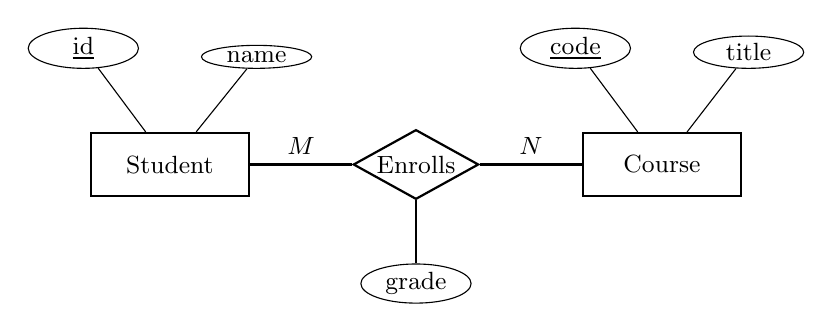
\begin{tikzpicture}[
  node distance=8mm and 13mm,
  every node/.style={font=\small},
  entity/.style={draw, thick, minimum width=20mm, minimum height=8mm},
  relation/.style={diamond, draw, thick, aspect=1.8, inner sep=1pt},
  attribute/.style={ellipse, draw, minimum width=14mm, inner sep=1pt},
]
  \node[entity] (student) {Student};
  \node[relation, right=of student] (enrolls) {Enrolls};
  \node[entity, right=of enrolls] (course) {Course};
  \node[attribute, above=of student, xshift=-11mm] (sid) {\underline{id}};
  \node[attribute, above=of student, xshift=11mm] (sname) {name};
  \node[attribute, above=of course, xshift=-11mm] (code) {\underline{code}};
  \node[attribute, above=of course, xshift=11mm] (title) {title};
  \node[attribute, below=of enrolls] (grade) {grade};

  \draw[thick] (student) -- node[above] {$M$} (enrolls) -- node[above] {$N$} (course);
  \foreach \a/\b in {student/sid, student/sname, course/code, course/title, enrolls/grade}
    \draw (\a) -- (\b);
\end{tikzpicture}
